\subsection{Circuito RL}\label{sec: RL}
\paragraph{}
En esta sección, se estudió la respuesta de un circuito RL en su régimen transitorio. Para lograr esto, se utilizó la configuración representada en la figura \ref{esq: RL}, con un inductor de $L=\SI{999(9)e-3}{H}$. Se alimentó el circuito con ondas cuadradas para conocer el comportamiento de la corriente cuando se utiliza una inductancia y determinar el tiempo característico $\tau_2$ del sistema. 
\paragraph{}
Se realizó un barrido de resistencias de $\SI{500(5)}{\Omega}$ a $\SI{5000(50)}{\Omega}$ para determinar la relación entre $\tau$ y $R$. Para esto, se registró la tensión en función del tiempo y se ajustó por la ecuación \eqref{eqn:RL} y se determinó $\tau$ para cada valor de resistencia. En la figura \ref{fig:RL 500} se encuentra un ejemplo de este ajuste, cuando $R=\SI{500(5)}{\Omega}$.
\begin{figure}[H]
    \centering
    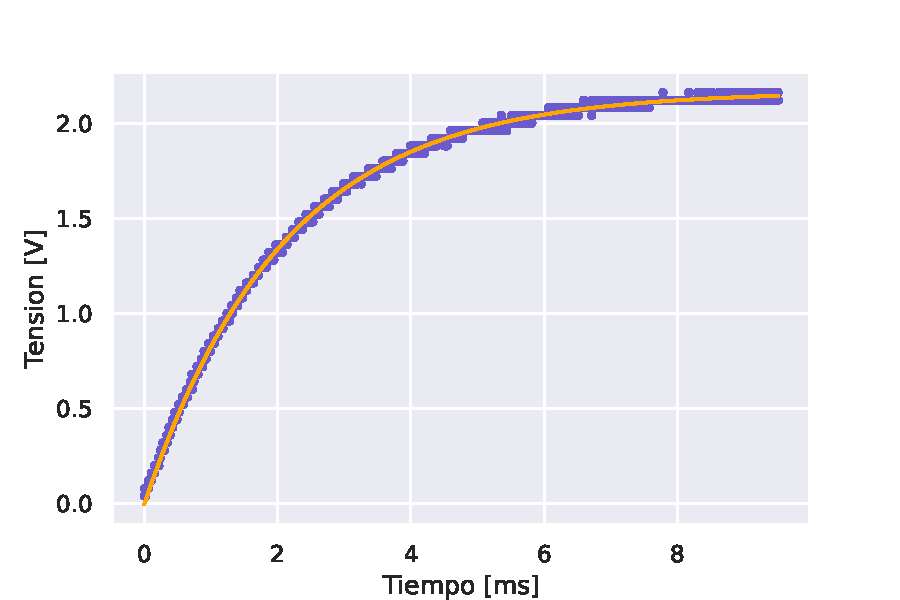
\includegraphics[scale= 0.7]{Figuras/RL/RL 500.pdf}
    \caption{Gráfico de la caída de tensión en el circuito RL con $R=\SI{500(5)}{\Omega}$. Los residuos presentan una distribución aleatoria}
    \label{fig:RL 500}
\end{figure}
\paragraph{}
En este caso representativo, el modelo representa correctamente los datos. Entonces, este método es válido para calcular $\tau_2$ mediante la \eqref{eqn:tau 2}. En la figura \ref{fig:RL tau R}, se muestra la relación entre $\tau_2$ y $R$. Se realizó un ajuste lineal con la ecuación \eqref{eqn:tau 2} y se determinó la pendiente, que es $1/L$
\begin{figure}[H]
    \centering
    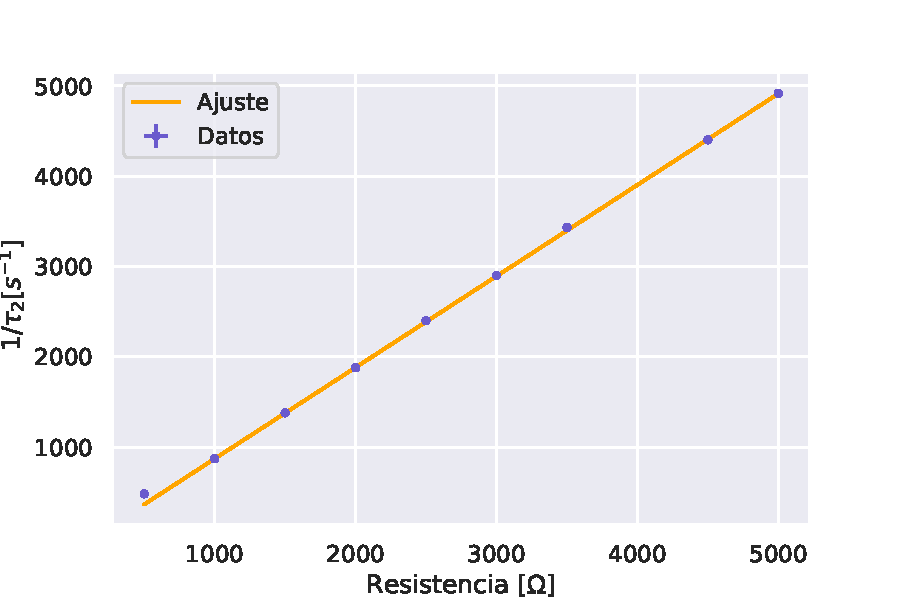
\includegraphics[scale=0.7]{Figuras/RL/tau RL.pdf}
    \caption{Gráfico de $1/\tau_2$ en función de $R$. Los residuos del ajuste presentan una distribución aparentemente aleatoria.}
    \label{fig:RL tau R}
\end{figure}
\paragraph{}
Se obtuvo un valor para la inductancia de $L=\SI{989(2)e-3}{H}$, lo cual es consistente con la inductancia medida directamente.

